\section{\MBSim - Program Overview}
\MBSim{} is written in the object-orientated programming language C++. 

Fig.~\ref{fig:objects} shows a class diagram.
\begin{figure}
	\centering
  	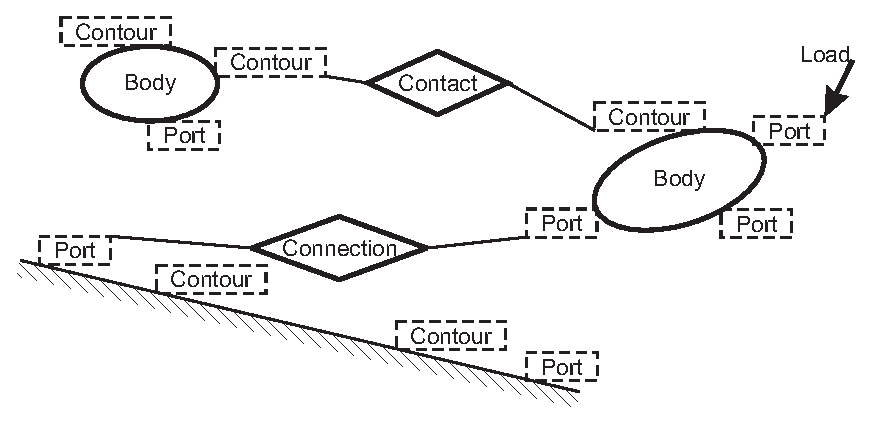
\includegraphics[width=12cm]{Figures/objectorientationMBSim.eps} % TODO
  	\caption{object structure in \MBSim}
  	\label{fig:objects}
\end{figure}

\subsection{Description of the Components}
The following classes can be used for modelling and simulating dynamical systems in \MBSim{}.

\subsubsection{Frames}

\subsubsection{Rigid Bodies}
To describe the kinematics and the update of further frames at rigid bodies a body-fixed frame has to be defined in \texttt{RigidBody} based on a predefined frame \texttt{"C"} in the centre of gravity. The frame for kinematics is updated with respect to a reference frame and its individual degree of freedom or its constrained relative motion. Both absolute and relative kinematical structures are canonically given by this frame recursion depending on the properties of the reference. The drawback of this general description is a time-dependent mass-matrix. A constant mass evaluation can be enforced by a boolean \texttt{"cb"}.\\
If there is a frame given tree structure a \texttt{Tree} for the kinematical evaluations is defined automatically.
%In jedem Fall sind Masse (\emph{setMass}), Tr\"agheitstensor bez. dem Bezugspunkt (\emph{setInertia}), generalisierte Koordinaten (\emph{setJT}, \emph{setJR}), evtl. Anfangsverformungen (\emph{setWrOK0}, \emph{setAWK0}) und \AMVis{}-Darstellungen (\emph{setAMVisBody}) anzugeben und die K\"orper dem MKS hinzuzuf\"ugen (\emph{addObject}). Auch ganze MKS k\"onnen als Slave einem Master-MKS hinzugef\"ugt werden.

\subsubsection{Flexible Bodies}
The equations of motion of a \texttt{FlexibleBody} is at the moment always derived with respect to a stationary frame. So, flexible bodies can only be used as root but not leave in a recursive tree structure. The following flexible bodies are available. 

\begin{itemize}
%\item \emph{BodyFlexible1s01Torsion}
%\item \emph{BodyFlexible1s21ANCF} 2D-Balken mit Absolute Nodal Coordinate Formulation
\item[] \texttt{BodyFlexible1s21RCM}\\
  planar beam using redundant coordinate methode with three coordinates per finite element node, translation  $x$, $y$ and rotation $\gamma$, as well as two additional bending deflections $c_1$, $c_2$
\item[] \texttt{BodyFlexible1s33RCM}\\
  spatial beam using redundant coordinate methode with six coordinates per finite element node, translation  $x$, $y$, $z$ and reversed Cardan rotation $\alpha$, $\beta$, $\gamma$, as well as four additional bending deflections $c_1$, $c_2$, $c_3$, $c_4$
%\item \emph{BodyFlexible1s23BTA} Biege-Torsions-Welle (5-Koordinaten pro Knoten $\alpha$, $y$, $\gamma$, $z$, $\beta$ im jeweils mit $\alpha$ mitdrehenden KOSY)
%\item \emph{BodyFlexibleLinearExternal}
\end{itemize}
%F\"ur die RCM-Modelle sowie die Biege-Torsions-Welle kann eine \AMVis-Darstellung
%(\emph{createAMVisBody}) aktiviert werden. Die Finiten Elemente selbst basieren im Fall von \emph{BodyFlexible1s21RCM}, \emph{BodyFlexible1s23BTA} und \emph{BodyFlexibleLinearExternal} auf einem neugeschaffenem Interface \emph{DiscretizationInterface} zur einheitlichen Darstellung.
%
%\subsubsection{Joints}
%Verbindungen werden ohne Reibung \"uber Ports (\emph{addPort}, \emph{connect}) an K\"orper bez. an die Umgebung angeschlossen. Dann ist auszuw\"ahlen, ob eine flexible Verbindung (\emph{ConnectionFlexible}) oder eine Starrk\"orperverbindung (\emph{ConnectionRigid}) zwischen K\"orpern oder eine externe Erregung (\emph{Load}) zur Modellierung verwendet werden soll. Der Freiheitsgrad der Verbindung wird \"uber \emph{setForceDirection} bez. \emph{setMomentDirection} angegeben. Dem MKS wird eine Verbindung anschlie"send \"uber \emph{addLink} mitgeteilt. \"Uber \emph{Link} kann auch eine Visualisierung der Verbindungskr\"afte (\emph{Arrow}) und der Kopplung selbst zugeschaltet werden; hierbei ist es m\"oglich zwischen einer Einheitenumrechnung und einer L\"angenvisualisierung zu unterscheiden (\emph{setScaleFactor}, \emph{setArrowHead}, \emph{setDiameter}), sowie den Partner f\"ur das Pfeilende festzulegen. Bei \emph{Load} wird mit \emph{setSignal} eine benutzerspezifische Funktion\footnote{\emph{UserFunction} gibt es bereits mit harmonischen (\emph{FuncHarmonic}), linearen Verlauf (\emph{FuncLinear}), oder auch als mehrdimensionale st\"uckweise Polynominterpolation (\emph{MDPPolynom})} vorgegeben.
%
\subsubsection{Contacts and Impacts}
Contacts and impacts are managed by \texttt{Contact}.\par 
The relative kinematics is defined between \texttt{Contour} classes. Thereby kinematically there might be a finite number of possible contact points; for the evaluation of force laws a decision rule has to be implemented. On velocity level the contact kinematics is independent of the specific contour. For the calculations on position level the following contours are available.
\begin{itemize}
\item[] \texttt{Point}\\
    most primitive rigid contour
\item[] \texttt{Plane}\\
    affine two dimensional surface
\item[] \texttt{Sphere}\\
    two dimensional sphere
\item[] \texttt{FlexibleBand}\\
    flexible contour describing a band in a certain distance and direction of a neutral fibre
\end{itemize}

Available contact kinematics on position level:
\begin{itemize}
\item[] \texttt{PointPlane}
\item[] \texttt{PointFlexibleBand}
\item[] \texttt{SpherePlane}
\end{itemize}

Concerning the constitutive laws it is distinguished between contact laws on acceleration and impact laws on velocity level. Further, both flexible and rigid laws in normal and tangential direction are available.\footnote{Modelling hint: There are contradictions between energy conservation in normal direction and dissipation due to friction when combining these features.})\par

For modelling own contact kinematics and constitutive laws some conventions are important.
\begin{itemize}
\item[] accompanying contour trihedral\\
    the first column is the outward pointing normal, 
\end{itemize}

%Linie-Contour1s, Kugel-Ebene, Kugel-Kugel und Kugel-Kegelstumpf. Auch Erweiterungen
%k\"onnen \"uber die Definition neuer Konturen und zugeh\"origer Kontaktkinematiken
%(\emph{setContactKinematics}) definiert werden. Hierzu ben\"otigt eine Kontur die
%Parametrisierung einer nach innen gerichteten Normale, einer Tangente, einer Position,
%einer Geschwindigkeit und einer Winkelgeschwindigkeit. Die Kontaktkinematik muss in einem
%ersten Schritt Normalabstand und Konturparameter \"uber eine Nullstellenfunktion
%bestimmen, sowie tangentiale Richtungsinformationen f\"ur Reibung in einem zweiten
%Schritt. Die Reihenfolge des \emph{connect}-Aufrufs muss dar\"uberhinaus behandelt
%werden.
%
\subsubsection{Integration Schemes}
Available integration schemes:
\begin{itemize}
\item[] \texttt{DOPRI5Integrator}\\
    Dormand-Prince one-step integration scheme of order 5 for nonstiff ODE with step size control
\item[] \texttt{RADAU5Integrator}\\
    one-step integration scheme of order 5 for stiff ODE with step size control
\item[] \texttt{TimeSteppingIntegrator}\\
    one-step integration scheme of order 1 for nonstiff MDE
\end{itemize}
%DAEs behandeln \emph{RADAU5DAEIntegrator}, \emph{DASKRIntegrator} und \emph{DASPKIntegrator}. Dar\"uberhinaus gibt es noch \emph{RKSuite}, \emph{LSODAR} (Mehrschrittverfahren steif/nicht steif) und \emph{LSODE}.  oder der allgemeinere \emph{ThetaTimeSteppingIntegrator} mit konstanter Schrittweitenvorgabe angewendet werden. \emph{TimeSteppingSSCIntegrator} implementiert f�r den semi-impliziten Fall eine Schrittweitensteuerung und \emph{DAETSIntegrator} liefert eine Kopplung zwischen TimeStepping und Dassl. Bei letzteren muss der Befehl \texttt{setSolver} vor der Initialisierung des MBS durchgef\"uhrt werden. Folgende M\"oglichkeiten stehen zur Wahl:

Available constraint equation solution schemes:
\begin{itemize}
\item[] \texttt{GaussSeidel}\\
    Gauss-Seidel solution scheme for piecewise linear systems (planar Coulomb friction)
\item[] \texttt{FixedPointSingle}\\
    Gauss-Seidel solution scheme with fixed point search and relaxation strategy for spatial Coulomb friction
\item[] \texttt{RootFinding}\\
    damped and globalised Newton scheme for spatial Coulomb friction
\end{itemize}
%\begin{itemize}
%\item Invertierbare Gleichungssysteme (GS) mit nur bilateralen Bindungen\\
%\emph{LinearEquations}: Cholesky-Verfahren
%
%
%\item Nichtlineare GS (3D-Coulomb-Reibung)\\
%  (\emph{setStrategy} mit \emph{local}/\emph{global})\\
%\emph{FixedPointTotal}: Jacobi-Verfahren mit Fixpunktsuche und R-Faktor-Strategie (verh\"alt sich zumeist schlechter als \emph{FixedPointSingle})\\  
%\emph{RootFinding}: ged\"ampftes, z.B durch Regula Falsi generalisiertes Newton-Verfahren mit
%  R-Faktor-Strategie (unstetige Jacobi-Matrix) und f\"ur unterbestimmte LGS ausw\"ahlbarer \emph{setLinalg} (LUDecomposition, LevenbergMarquardt, PseudoInverse) (f\"ur schlecht konditionierte Dylassus-Matrix meistens am besten)
%\end{itemize}
%Der Befehl \emph{stopifnoConvergence(\texttt{true},\texttt{true})} zwingt den Integrator abzubrechen, falls keine Konvergenz vorliegt, und die Kontaktsituation auszugeben.
%

\subsection{Program Flow}
Conceptionally the program flow is defined by the election of the integration scheme. It can always be stopped using \texttt{Ctrl-C}.

\subsubsection{Timestepping Integration}
Timestepping integration solves the whole equations of the system including the contacts on velocity level with fixed time step size. In detail one has the following work flow.
\begin{enumerate}
\item $\text{\texttt{DS::plot}}\left(t,\vq,\vu\right)$
\item $\vq\leftarrow\vq+\text{\texttt{DS::deltaq}}\left(t,\vq,\vu\right)$
\item $t\leftarrow t+\Delta t$
\item $\text{\texttt{DS::update}}\left(t,\vq,\vu\right)$
    \begin{enumerate}
    \item[]\texttt{DS::updateStateDependentVariables}\\
      update variables depending on the generalised state and the structure of the system with one independent group and several trees
    \item[]\texttt{DS::updateg}
      \begin{itemize}
      \item update of the relative position kinematics independent of the system structure using the order
      \begin{align*}
        \text{\texttt{Link}}\rightarrow\text{\texttt{LinkMechanics}}\rightarrow\text{\texttt{Joint}, \texttt{Contact}, \texttt{Actuator}}\rightarrow\text{\texttt{ContactKinematics}}
      \end{align*}
      \item several contacts points are possible from the kinematical point of view, whereby the maximum number is calculated in \texttt{ContactKinematics}\\
      \item conventions in the contact frame matrix:
        \begin{itemize}
        \item frames are cartesian
        \item first column is the outpointing normal
        \item second column sign is different for the two contacting bodies 
        \end{itemize}
      \end{itemize}
    \item[]\texttt{DS::checkActiveg}
      \begin{itemize}
      \item determine the state of the relative kinematics concerning the activity of links
      \item redefine global memory references using indices and indents
      \end{itemize}
    \item[]\texttt{DS::updategd}
      \begin{itemize}
      \item update of the relative velocity kinematics independent of the system structure
      \item can be done in the child classes of \texttt{LinkMechanics}
      \end{itemize}
    \item[]\texttt{DS::updateT}\\
      updates the linear transformation matrix $\dot{\vq}=T\vu$ independent of the system structure
    \item[]\texttt{updateJacobians}\\
      updates the \textsc{Jacobians} for projecting forces in generalised directions dependent on the system structure
    \item[]\texttt{updateh}\\
      updates the right hand sides with the possibility to account for internal forces of \texttt{objects} and external forces of \texttt{links} independent of the system structure
    \item[]\texttt{updateM}\\
      updates the mass matrix independent of the system structure
    \item[]\texttt{facLLM}
      \begin{itemize}
      \item computes the \textsc{Cholesky} decomposition of the mass matrix dependent on the system structure
      \item \texttt{group} calculates the matrix inverse locally per object
      \item \texttt{tree} calculates the matrix inverse globally
      \end{itemize}
    \item[]\texttt{updateW}\\
      updates the \textsc{Jacobian} between in general set-valued \texttt{link}-force parameters and generalised coordinates
    \item[]\texttt{updateV}
      \begin{itemize}
      \item the decomposition of the in general set-valued \texttt{link}-forces
      \begin{align*}
      \vW\vlambda=\vW_N\vlambda_N+\vW_T\vlambda_T
      \end{align*}
      in a normal and tangential part allows to separate the single-valued slip case
      \item for affected \texttt{links} it is
      \begin{align*}
      \tilde{\vW}\tilde{\vlambda}=\left(\tilde{\vW}_N+\mu\tilde{\vW}_T\right)\tilde{\vlambda}_N=\tilde{\vV}\tilde{\vlambda}_N\ .
      \end{align*}
      \item altogether this is a reduction of the set-valued equations being expressed by the projection
      \begin{align*}
      \vV\vlambda^{*}\ .
      \end{align*}
      \end{itemize}
    \item[]\texttt{updateG}
      \begin{itemize}
      \item the force action matrix
      \begin{align*}
      \vG=\vW^T\vM^{-1}\vV
      \end{align*}
      must be calculated by the most global view, namely the \texttt{DynamicSystemSolver}
      \item the size of $\vG$ is reduced due to the introduction of $\vV$ but is non-symmetric
      \item for a time-stepping scheme it is $\vV=\vW$
      \end{itemize}
    \end{enumerate}
\item $\text{\texttt{DS::solveImpacts}}\left(t,\vq,\vu\right)$
    \begin{itemize}
    \item the constrained equations are solved on velocity level using sparse matrix structures (cf.~\cite[MKL sparse matrix storage format]{Intel08})
    \item block structures are not evaluated
    \end{itemize}
\item $\vu\leftarrow\vu+\text{\texttt{DS::deltau}}$
\item $\vx\leftarrow\vx+\text{\texttt{DS::deltax}}$
\item \texttt{DS::projectGeneralizedPositions}
\end{enumerate}

\subsubsection{Event-Driven Integration}
Currently, \texttt{LSODAR} is the only event-driven integrator with automatic switch between stiff and non-stiff equations.
\begin{enumerate}
\item \texttt{DS::computeInitialCondition}\\
    checks for system configuration and creates the necessary contact container
\item $\text{\texttt{DS::plot}}\left(t,\vq\right)$
\item \texttt{DLSODAR} 
    \begin{enumerate}
    \item[]$\text{\texttt{DS::zdot}}\left(t,\vq,\vu\right)$ is available for standard and inverse kinetics calculations
      \begin{itemize}
      \item \texttt{wb} means $\bar{w}$ and describes the acceleration terms in the constraint kinematics
      \item \texttt{computeConstraintForces} uses a least square algorithm to solve the Delassus equations, assume $Ax=b$ with a $m\times n$ full-rank matrix $A$, then there are two cases
        \begin{itemize}
        \item $m\geq n$ (skinny) can always be solved by $\left\|Ax-b\right\|\rightarrow\min$ and so by SVD\\
          analytically the solution is given by the normal equations $x=\left(A^TA\right)^{-1}A^Tb$
        \item $m<n$ (fat) has an infinite dimensional solution space, one has to pick one solution\\
          $\left\|x\right\|\rightarrow\min,\ Ax=b$ which is analytically given by $x=A^T\left(A^TA\right)^{-1}b$, again numerically a SVD solves the problem most efficiently
        \end{itemize}
      \end{itemize}
    \item[]\texttt{DS::getsv} the stop vector defines the root function concerning contacts and stick-slip-transitions for the DAE solver
      \begin{itemize}
      \item it can be only set by \texttt{Link}
      \item contains kinematics for not-active directions and kinetics for active directions
      \item the last entry is used for position and velocity projections
      \end{itemize}
    \end{enumerate}
\item \texttt{DS::shift} is invoked, if there is a sign change in the stop vector
    \begin{itemize}
      \item drift compensation if indicated by stop vector
      \item project to slighly positive gaps to avoid instantaneous appearance of new shift point
      \item[] \texttt{updateCondition} should impact or differential equations be solved, after earlier mentioned reconfiguring
      \item case studies
        \begin{itemize}
        \item[] \texttt{impact} has highest priority and changes overall configuration
        \item[] \texttt{impact} requires \texttt{D::checkAllgd} because of possible slip-stick transition
        \item no difference between $\Lambda$ and $\lambda$
        \item \texttt{gdn} means $\dot{g}^{+}$
        \item[] \texttt{impact} involves new configuration and so also the equations of motion have to be solved
        \item \texttt{checkActivegdd} has to be done with the same tolerance like in the nonlinear equations solver
        \item[] \texttt{gActive} means a contact is closed
        \item[] \texttt{gdActive} means a contact remains closed
        \end{itemize}
    \end{itemize}
\end{enumerate}

%exemplarisch ein System aus Umwelt und zwei K�rpern. Angedeutet sind Wechselwirkungen
%dieser untereinander �ber Kontakte und Verbindungen sowie eine �u�ere Last.
%
%Ein K�rper~(\texttt{Body...}) ist in \MBSim{} durch seine Lagen~$\vq$ und
%Geschwindigkeiten~$\vu$ parametrisiert. Die Parameter der beschreibenden
%Differentialgleichung sind bei starren K�rpern~(\texttt{BodyRigid...}) immer Masse~$m$ und
%Tragheitstensor~$\vTheta$. Die Modelle f�r flexible K�rper~(\texttt{Bodyflexible...}) sind in der
%Parametrisierung jeweils sehr speziell -- f�r sie sei auf die jeweiligen Implementierungen
%und die zugeh�rigen Dokumentationen verwiesen.
%
%Die Umwelt kann wie auch alle K�rper Konturen~(\texttt{Contour}) sowie
%Anschl�sse~(\texttt{Port}) aufnehmen, auf denen Kontakte sowie diskrete Wechselwirkungen
%definiert werden k�nnen. Zudem ist Gravitation �ber die Umwelt definiert.
%
%Kontakte zwischen den Konturen unterschiedlicher K�rper k�nnen sowohl als
%Starrk�rperkontakt~(\texttt{ContactRigid}, mengenwertig, nicht-glatte Dynamik) als auch
%als nachgiebiger Kontakt~(\texttt{ContactFlexible}, funktional, lokale Steifigkeit)
%definiert werden. Reibung wird hierbei jeweils durch die Angabe der auszuwertenden
%Reibrichtungen eingebunden. Verbindungen zwischen zwei Anschl�ssen k�nnen sowohl starr
%(\texttt{ConnectionRigid}) als auch mit Nachgiebigkeit~(\texttt{ConnectionFlexible})
%modelliert werden. F�r �ussere Lasten~(\texttt{Load}) k�nnen beliebige Vorschriften
%angegeben werden.
%%%------------------------------------------------------------ SUBSECTION --
%\subsection{Hinweise}
%\begin{enumerate}
%  \item F\"ur Anwendungen die MBSim-Ableitungen verwenden, muss im \texttt{Makefile} der
%       \texttt{pkg}-Aufruf ge\"andert werden zu \texttt{mbsimMechAdd} oder Adequates, um
%       die Bibliotheken einzubinden.
%  \item In \emph{Vec}-Schreibweise d\"urfen nur Ziffern auftreten
%  \item Parametrisierung der Gesamtbewegung (siehe Skriptum \cite{Foer07}) mit $\vA_{K_0K}$ durch $\vq$ und mit direkt vorgebbarem $\vA_{WK_0}$
%  \item Plotlevel (0,1,2,3) erh\"oht f\"ur jedes Element extra die Ausgabedateigr\"o"se (z.B. zus\"atzlich Kontaktgeschwindigkeiten); f�r AMVis ist ein Wert gr��er als 0 n�tig.
%  \item Projektionen zur Korrektur bei Verletzung von Lage-Nebenbedingungen sind bei Time-Steppern \"uber \emph{setDriftCompensation} m\"oglich. Bei der Interpretation ist
%       allerdings der Drift vom Diskretisierungsfehler (Time-Stepper ist 1. Ordnung) zu
%       unterscheiden; bei Kontaktdurchsinken sollte demnach zun\"achst die Schrittweite
%       verkleinert werden. Bei h\"ochstens Gleichungsnebenbedingungen k\"onnen bei reinen
%       Starrk\"orpersystemen auch alle anderen
%       Integratoren verwendet werden, da das System dann intern auf Beschleunigungsebene gebracht
%       wird, bei flexiblen K\"orpern ist dies nur zum Teil der Fall. Auch f\"ur Integratoren
%       h\"oherer Ordnung entsteht also ein numerischer Drift. Zur Vermeidung von numerischen
%       Fehlern ist es h\"aufig besser, Gleichungsnebenbedingungen
%       durch relativkinematische Beschreibungen zu ersetzen.
%  \item Es besteht die M\"oglichkeit von negativen Abst\"anden bis zur Kontaktdetektion, da die Kontakte mit Toleranzen versehen sind (zur Behebung ist die Schrittweite manuell zu verringern).
%  \item Bei unterbestimmten GS sind Kr\"afte au"serhalb der Bewegungsebene m\"oglich, solange die Physik nicht verletzt wird. Eine Addition aller Kr\"afte ergibt hierbei die korrekte Gesamtkraftwirkung. Alternativ k\"onnen \emph{flexibleLinks} oder z.B. bilaterale Links verwendet werden, die passive Kr\"afte eindeutig berechnen. Die Modellierung in MBSim ist im Wesentlichen gleich, jedoch kann dann wieder das Newton-Verfahren mit LU-Zerlegung als Solver benutzt werden. Z.B. im Reibungsfall sind solche alternativen Modellierungen zur Vermeidung mathematischer Abh\"angigkeiten nicht m\"oglich. Hier muss also ein iterativer L\"oser verwendet werden. Eine Konvergenzanalyse ist dann allerdings nicht m\"oglich.
%  \item Standardm\"assig werden die Kontaktkr\"afte nur im aktiven Fall aktualisiert, um den Vorg\"angerwert zur schelleren Konvergenz auszunutzen. Mit \emph{setUseOldla} kann dies unterbunden werden.
%  
%  \item Kontakte m\"ussen f\"ur jeden K\"orper extra definiert werden, um die Physik jeweils gleich zu behandeln.
%  \item Der Zustand kann f�r \emph{Tree} derzeit nicht ausgegeben werden.
%\end{enumerate}

%%------------------------------------------------------------ SUBSECTION --
\subsection{Plot Routines}\label{sec:plot}

\subsubsection{Usage}
For getting data from \MBSim{} a \HDF{} wrapper is used. Viewing the multibody system parts can be done with
\begin{verbatim}
    h5lsserie <h5-file>
\end{verbatim}
Several possible options are explained by typing \texttt{-h}:
\begin{enumerate}
\item[\texttt{-d}] shows the description of the data to plot\\
\item[\texttt{-l}] shows the column labels of the data to plot\\
\item[\texttt{-f}] follows external links in a set of \HDF{}-files to avoid redundant data (\HDF{} is possible per DynamicSystem)
\end{enumerate}
The specific names in \HDF{} format are specialised by reading from right to left. The url to specific data is given by a path and can be used in
\begin{verbatim}
    h5dumpserie <path>
\end{verbatim}
The column one is interested in is declared using a colon. Also several columns can be appended, whereby shorter ones are enlarged by \texttt{nan} entries. Altogether, it is possible to use the dump by
\begin{verbatim}
    gnuplot "<dump" u *:* w l
\end{verbatim}
or in \textsf{MatLab} by
\begin{verbatim}
    h5dump('<path>')
\end{verbatim}

\subsubsection{Implementation}
In \MBSim{} plotting is done using \texttt{plotFeatures} being defined in \texttt{element.h} and set in \texttt{dynamic\_system\_solver.cc}. One plot-file comprises time-series of rowvectors with the same data type in all entries.

